\documentclass[10pt]{article}

% Lines beginning with the percent sign are comments
% This file has been commented to help you understand more about LaTeX

% DO NOT EDIT THE LINES BETWEEN THE TWO LONG HORIZONTAL LINES

%---------------------------------------------------------------------------------------------------------

% Packages add extra functionality.
\usepackage{
	times,
	graphicx,
	epstopdf,
	fancyhdr,
	amsfonts,
	amsthm,
	amsmath,
	algorithm,
	algorithmic,
	xspace,
	hyperref,
	multirow,
	tabularx,
	}
\usepackage[left=1in,top=1in,right=1in,bottom=1in]{geometry}
\usepackage{sect sty}	%For centering section headings
\usepackage{enumerate}	%Allows more labeling options for enumerate environments 
\usepackage{epsfig}
\usepackage[space]{grffile}
\usepackage{booktabs}
\usepackage{amsmath}
\usepackage[super]{nth}
\usepackage{array}
\usepackage{graphicx}
\usepackage{enumerate}
\usepackage{alltt}
\usepackage{fancyvrb}
% This will set LaTeX to look for figures in the same directory as the .tex file
\graphicspath{.} % The dot means current directory.

\pagestyle{fancy}

\lhead{\YOURID}
\chead{\MyLang: Language Specification}
\rhead{\today}
\lfoot{CSCI 334: Principles of Programming Languages}
\cfoot{\thepage}
\rfoot{Spring 2022}

% Some commands for changing header and footer format
\renewcommand{\headrulewidth}{0.4pt}
\renewcommand{\headwidth}{\textwidth}
\renewcommand{\footrulewidth}{0.4pt}

% These let you use common environments
\newtheorem{claim}{Claim}
\newtheorem{definition}{Definition}
\newtheorem{theorem}{Theorem}
\newtheorem{lemma}{Lemma}
\newtheorem{observation}{Observation}
\newtheorem{question}{Question}

\setlength{\parindent}{0cm}
%---------------------------------------------------------------------------------------------------------

% DON'T CHANGE ANYTHING ABOVE HERE

% Edit below as instructed
\newcommand{\MyLang}{1 e + a}	% Replace MyLang with your language name #
\newcommand{\PartnerOne}{Valeria Starkova}	% Replace PartnerOne with your name #
\newcommand{\YOURID}{\PartnerOne{}} % Remove \PartnerTwo if working alone.


\title{\MyLang: Language Specification}
\date{Spring 2022}
\author{\PartnerOne{}} % Remove \PartnerTwo if working alone.

\begin{document}
\maketitle

\vspace{\baselineskip}	% Add some vertical space
\graphicspath{ {./images/} }


\maketitle


\section{Introduction}


This language allows drummers to notate drums efficiently, without using inconvenient 
intermediary software. As it can be tedious to write drum tabs in UIs that are not designed 
for this purpose, this language lets users write drum tabs in a simple and intuitive way: 
by utilizing the good old "1 e and a" counting system. 

\item 
A drum part's structure is often constant throughout a song, with only slight variations 
across its parts (intro, verse, pre-chorus, chorus, bridge, etc.). This language also helps to 
avoid repetition by allowing the user to write one structure only once, then reuse it in other 
parts with slight modifications if necessary.

\section{Design Principles}
Writing sheet music for drums in this language is as easy as 1 e $+$ a!
The most important design principle in this language is that users can 
create and re-use patterns, bars, and beats that can be easily modified when writing the drum tabs. 
Further, the language has an online editor in which users can quickly write, test, and listen to
the beats they wrote.
Perhaps in the future, users will be able to share the source code for each song written in 
this programming language on a platform similar to GitHub, where they can keep track of 
their commits, collaborators, etc. 



\section{Examples}

\subsection{Example 1}
It is very easy to create a pattern, just by using the "1 e and a" counting system. 
We put separators \verb+|+ to disambiguate the division of the beats. Since patterns alone
cannot be rendered, we can put it inside a bar expression like this:
\begin{verbatim}
    time: 4/4
    division: 1/16
    tempo: 120
    title: example 1
    
    pattern sixteenth_notes: [1 e + a | 2  e + a  | 3 e + a  | 4  e + a  |]
    
    bar mybar:
      hh: [sixteenth_notes]
    
    render: { mybar }
\end{verbatim}

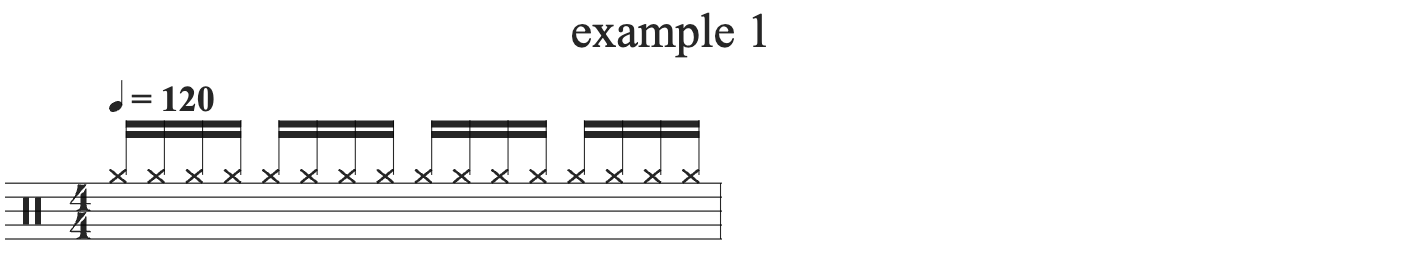
\includegraphics[scale=0.7]{Screenshot 2022-05-22 at 8.40.33 PM.png}


\subsection{Example 2}
Simple example of creating a two measure beat by providing two bar expressions in the render instruction.
\begin{verbatim}
    time: 4/4
    division: 1/16
    tempo: 120
    title: example 2
    
    pattern sixteenth_notes: [1 e + a | 2  e + a  | 3 e + a  | 4  e + a  |]
    
    bar intro:
      sn: [sixteenth_notes]
      bd: [1 | 2 | 3 | 4|]
      
    bar main:
      hh: [sixteenth_notes]
      sn: [1 | 2 | 3 | 4|]
    
      
    render: { intro, main } 
\end{verbatim}
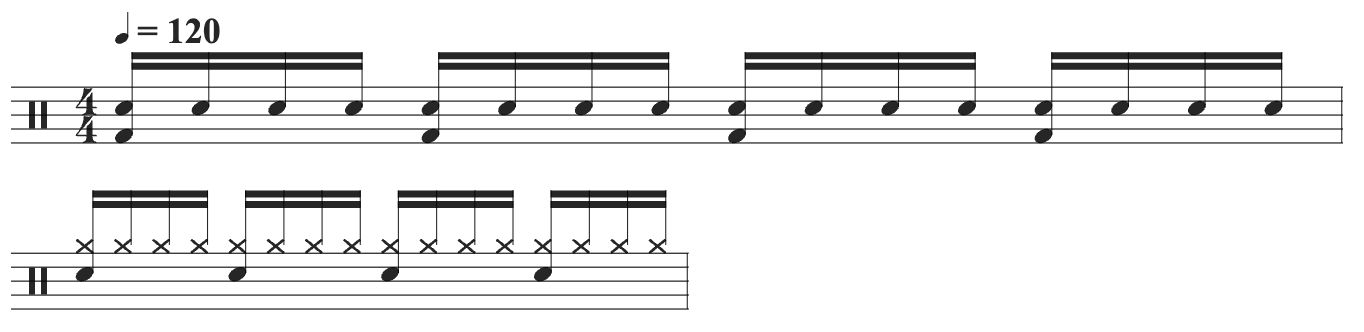
\includegraphics[scale=0.7]{Screenshot 2022-05-22 at 8.39.27 PM.png}

\subsection{Example 3}
Create a snippet by repeating the pre-defined measure and changing some of the drums and patterns on the last measure.
\begin{verbatim}
    time: 4/4
    division: 1/16
    tempo: 127
    title: Chop Suey!
    
    pattern eigthNotes: [1 + | 2 + | 3 + | 4 + |]
    pattern fourthNotes: [ 1 | 2 | 3 | 4 |]
    
    
    bar intro_bar:
      bd: [ fourthNotes ]
      t1: [ 1 + a | 2 | | |]
      t2: [ |  e + | 3 | |]
      ft: [ 1 | | e + a | 4 + |]
      
    snippet intro:
      change 8: intro_bar(8) {
        bd: [ eigthNotes ]
        sn: [  |  |  | + |]
        t1: [ 1 + | 2 + | 3 + | 4 |]
        t2: [ | | | |]
        ft: [ 1 + | 2 + | 3 + | 4 |]
      }
    
    render: { intro }
\end{verbatim}
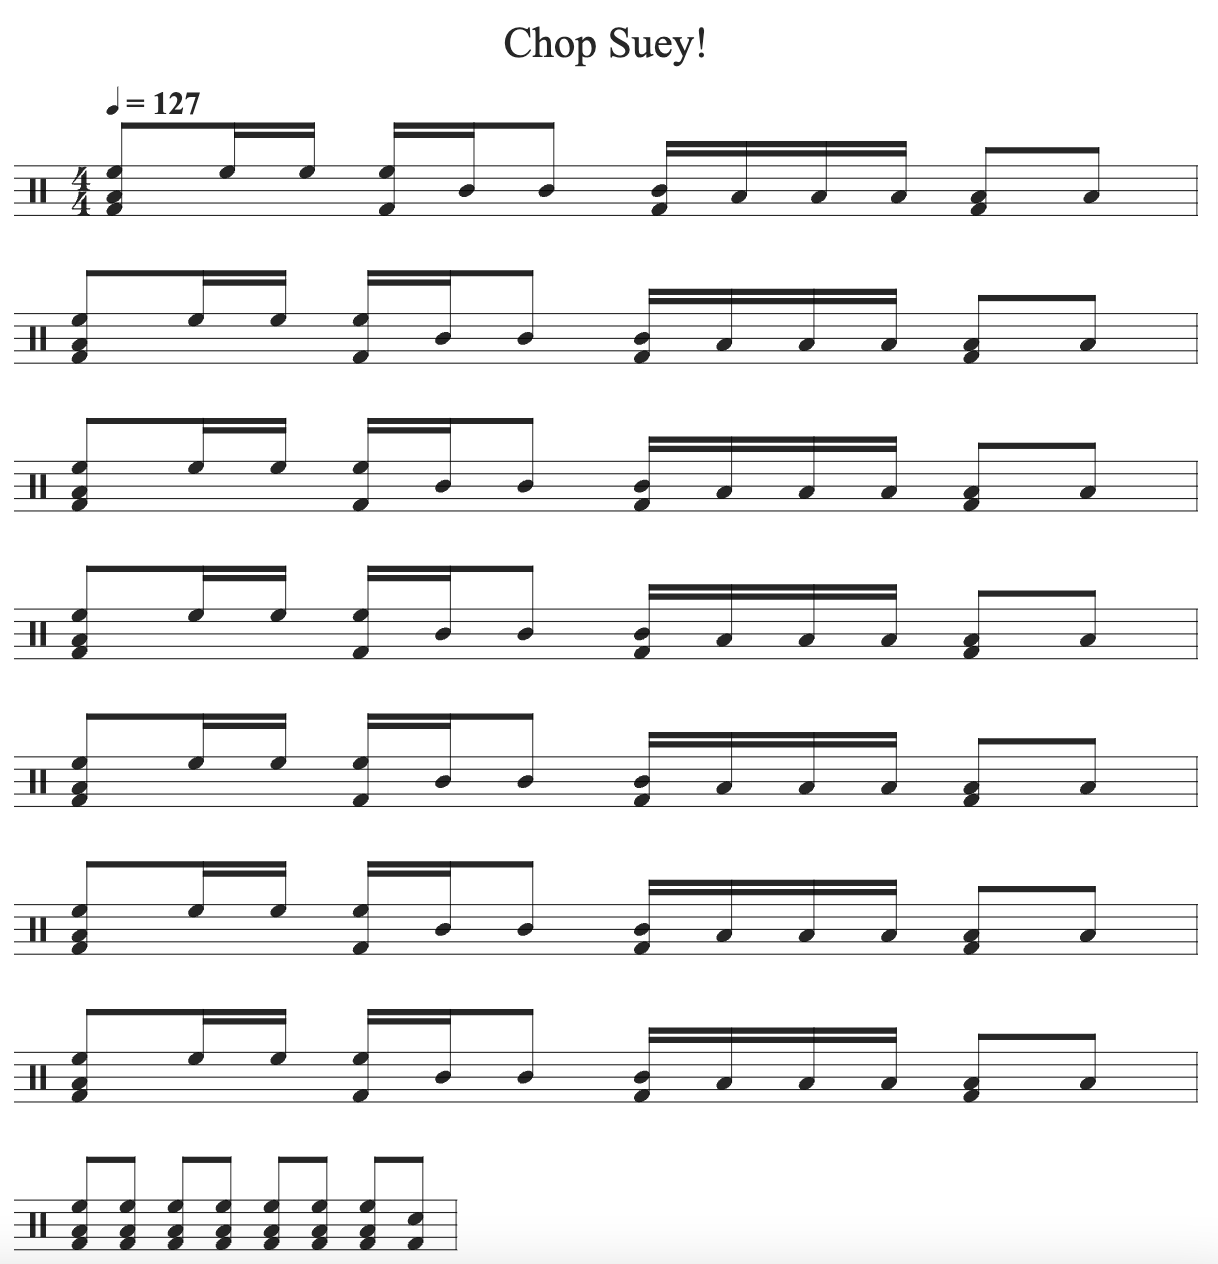
\includegraphics[scale=0.7]{Screenshot 2022-05-22 at 8.49.34 PM.png}

\section{Language Concepts}
There are two core concepts a user should understand in order to write programs in this language. First, how to notate different parts of the drumkit. Below is an example of a basic drumkit and the corresponding abbreviations we will use to write programs.

\begin{verbatim}
CC = Crash cymbal
HH = Hi-hat
RD = Ride cymbal
SN = Snare drum
T1 = High tom
T2 = Low tom
FT = Floor tom
BD = Bass drum
\end{verbatim}

Secondly, a user should be familiar with the “1 e and a” counting system:
\\\\
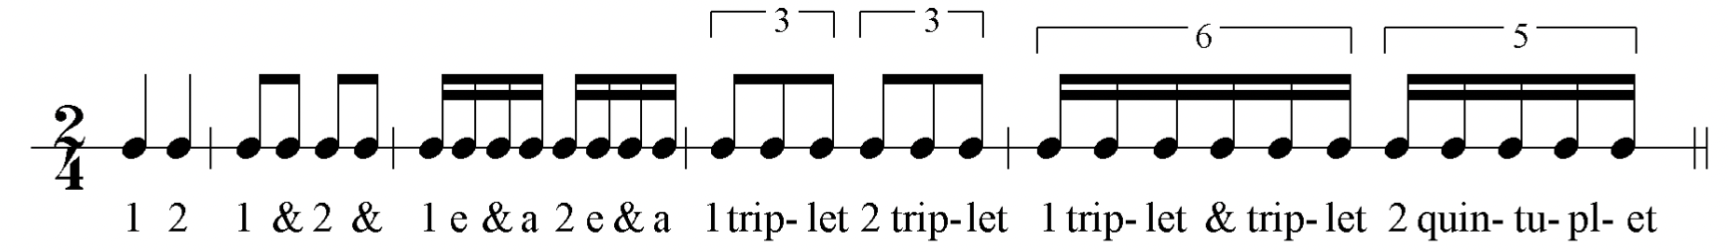
\includegraphics[scale=0.5]{img.png}

Now knowing this, we can assign patterns to each part of the drum kit. For example, in 4/4 time and 1/16 division, we can assign to SN (the snare drum) the pattern \verb+1 e | 2 e | 3 e | 4 a |+, where $|$ just symbolises division of the beat.


\section{Syntax}

A pattern is made up of notes. Patterns can be 
assigned to drums in a bar. Bars can be combined to create
a snippet. Bars inside a snippet can be repeated or modified inside 
a repeat or change instruction.

\begin{alltt}
    <num>           ::= x \ensuremath{\in} Z+
    <string>        ::= y \ensuremath{\in} { a . . . z }
    <varname>       ::= <string> | _

    <time>          ::= time: <num>/<num>
    <division>      ::= division: <num>/<num>
    <tempo>         ::= tempo: <num>
    <title>         ::= title: <string>
    <settings>      ::= <time> <division> <tempo> <title>

    <sep>               ::= |
    <note>              ::= <num> | e | + | a 
    <notes>             ::= <note>+
    <notes_with_sep>    ::= <notes><sep>
    <pattern>           ::= <notes_with_sep>+
    <pattern_expr>      ::= pattern <varname>: [<pattern>]
    
    <drums>                 := cc | hh | rd | sn | t1 | t2 | ft | bd | r
    <drum_pattern_var>      ::= <drums>: [<varname>]
    <drum_pattern_notes>    ::= <drums>: [<pattern>]
    <drum_pattern>          ::= <drum_pattern_var> | <drum_pattern_notes>
    <many_drum_patterns>    ::= <drum_pattern>+
    <bar_expr>              ::= bar <varname>: <many_drum_patterns>
    
    <repeat>                ::= repeat <num>: \ensuremath{\{}<varname>,+\ensuremath{\}}
    <change_every>          ::= every <num>
    <change_many>           ::= <num>,+
    <change_option>         ::= <change_every> | <change_many>
    <change>                ::= change <num>: 
                                <varname> (<change_option>)\ensuremath{\{}
                                    <drum_pattern>+
                                \ensuremath{\}}
    <snippet_data>          ::= <repeat> | <change>
    <snippet_expr>          ::= snippet <varname>: <snippet_data>+

    <render>                ::= render: \ensuremath{\{}<varname>,+\ensuremath{\}}

    <data_expr>             ::= <pattern_expr> | <bar_expr> | <snippet_expr>
    <many_data_expr>        ::= <data_expr>+
    <expr>                  ::= <settings> 
                                <many_data_expr> 
                                <render>
\end{alltt}

\section{Semantics}
\begin{tabularx}{1\textwidth} { 
  | >{\raggedright\arraybackslash}X
  | >{\centering\arraybackslash}X 
  | >{\centering\arraybackslash}X 
  | >{\centering\arraybackslash}X 
  | >{\raggedleft\arraybackslash}X 
  | >{\raggedleft\arraybackslash}X |
  | >{\raggedleft\arraybackslash}X |
  | >{\raggedleft\arraybackslash}X |
  | >{\raggedleft\arraybackslash}X |
  }
 \hline
 Syntax & Abstract Syntax & Type & Meaning \\
 \hline

    % x \in R  & x of int & int & x is a primitive \\
    % \hline
    time: 4/4 & Time of uint8 * uint8 & Settings & Top number tells how many beats should be in one measure, and
    the bottom number tells what value of note should get the beat. \\
    \hline
   
    division: 1/16 & Division of uint8 * uint8 & Settings & The minimum value that notes can divide into \\
    \hline

    tempo: 120 & Tempo of uint8 & Settings & The speed of the music to be played \\
    \hline

    title: My Title & Title of string & Settings & Title of the music \\
    \hline

    1 e + a \verb+|+ & Num of int \verb+|+ E \verb+|+  And \verb+|+  A \verb+|+ Sep & Note  & 
    A way of writing notes: 1 specifies a strong beat, e is a weak beat, + is a strong beat, 
    and a is a weak beat. Any of these notes (or even no notes at all), make up one beat. 
    As defined by the time signature above, if we combine 4 beats then we get one full measure (ex: 1 e + a 2 e + a 3 e + a 4 e + a).
    We put a separator \verb+|+ after each beat to disambiguate the division of the beats:
    1 e + a \verb+|+ 2 e + a \verb+|+ 3 e + a \verb+|+ 4 e + a \verb+|+\\


    \hline
    
    sn & Drum of \verb+|+ CC   \verb+|+ RD     \verb+|+ HH     \verb+|+ SN     \verb+|+ T1   \verb+|+ T2  \verb+|+ FT   \verb+|+ BD  \verb+|+ Rest 
    & Drum 
    & Denotes a drum \\
   \hline

    pattern varname: [1 \verb+|+ 2 e + a \verb+|+ 3 \verb+|+ 4 \verb+|+]
    & Pattern of PatternName * (Note list) 
    & Pattern 
    & A pattern is a data type that contains one measure of notes as defined by the time signature.\\
    \hline
     hh: [ string ]  & Drum * PatternName & DrumPatternVar & 
     Indirect way of assigning a pattern referenced by it's variable name to a drum \\
    \hline
     hh: [ 1 \verb+|+ 2 \verb+|+ 3 \verb+|+ 4 ] & Drum * (Note list) & DrumPatternNotes & 
     Direct way of assigning a pattern to a drum  \\
    \hline
     
    
     bar barName: \n
        hh: [1 \verb+|+ 2 \verb+|+ 3 \verb+|+ 4 \verb+|+] \n
        sn: [somePattern]
    
    & Bar of BarName * (DrumPatternVar list * DrumPatternNotes list) & Bar & 
    A bar is a data type that contains one or more pattern variable names or patterns assigned to drum instruments.\\
    \hline
    

\end{tabularx}

\begin{tabularx}{1\textwidth} { 
    | >{\raggedright\arraybackslash}X
    | >{\centering\arraybackslash}X 
    | >{\centering\arraybackslash}X 
    | >{\centering\arraybackslash}X 
    | >{\raggedleft\arraybackslash}X 
    | >{\raggedleft\arraybackslash}X |
    | >{\raggedleft\arraybackslash}X |
    | >{\raggedleft\arraybackslash}X |
    | >{\raggedleft\arraybackslash}X |
    }
   \hline
   Syntax & Abstract Syntax & Type & Meaning \\
   \hline
   repeat 2: { oneBar, twoBar }
    
    & Repeat of int * (BarName list) &
    SnippetData & 
    
   repeat instruction will repeat one or more bars a given number of times.
    \\
    
    \hline

     change 5: barName (1,2) \ensuremath{\{}  cc: [1 \verb+|+ 2 \verb+|+ 3 \verb+|+ 4 \verb+|+] \ensuremath{\}}   or \newline
     change 4: barName (every 2) \ensuremath{\{}  cc: [ patternName]\ensuremath{\}}
    
    & RepeatChange of int * BarName * RepeatOption * (DrumPattern list) &
    SnippetData & 
    
   repeat instructions repeat and also change a given bar as specified by the 
   option inside parens (every N-th bar or a given list of integers). The data
   to change the bar is written inside curly brackets, which are just drum->pattern assignments.
   \\
    
    \hline

    snippet mysnippet: \newline
        change ...\newline
        repeat ...\newline
    
    & Snippet of SnippetName * (SnippetData list) &
    Snippet & 
    
    Snippet is a data type that contains one or more combinations of the two possible instructions: repeat instruction, and change instruction.
   \\
   \hline
    render: \ensuremath{\{}  someBar, someSnippet, someBar, ...\ensuremath{\}} 
    
    & string list &
    Render & 
    
    The render keyword will render (or in other words, evaluate) the variables specified inside curly brackets {} after the semicolon :. The render keyword must always come the very last in the program.
   \\
   \hline

\end{tabularx}
\begin{enumerate}[i.]
    \item  A primitive value is a note defined by a counting value such as \verb+1+,  \verb+e+,  \verb#+#, \verb+a+. We put separators \verb#|# after each beat.
    \item Notes \verb+1+,  \verb+e+,  \verb#+#,  \verb+a+ are combined to create a \verb+pattern+:
    \begin{verbatim}
        pattern: [1 + | 2 e | 3 | 4 e + a|]
    \end{verbatim}
    A \verb+bar+ can be created by applying various \verb+pattern+s to different parts of the drumset (\verb+hh+, \verb+sn+, \verb+bd+, etc).
    \begin{verbatim}
        bar myBar: 
            sn: [1 + | 2 e | 3 | 4 e + a|]
            bd: [patternVar]
    \end{verbatim}
    And a \verb+snippet+ can be created by combining and/or repeating multiple \verb+bar+s. There 
    are 2 instructions which repeat a given bar(s): repeat without change and repeat with change. Repeat 
    without change just repeats one or more bars N times. Repeat with change (or simply \verb+change+)
    instruction changes one given bar on top of repeating it.
    \begin{verbatim}
        snippet mySnippet: 
            repeat 2: {myBarOne, MyBarTwo}
            change 6: MyBarTwo (every 2) {
                bd: [different_pattern]
            }
            change 16: MyBarTwo (1,6,8,9) {
                cc: [different_pattern]
                cc: [1|2|3|4|]
            }
    \end{verbatim}

    \item Diagram representation of my program:
    \\
    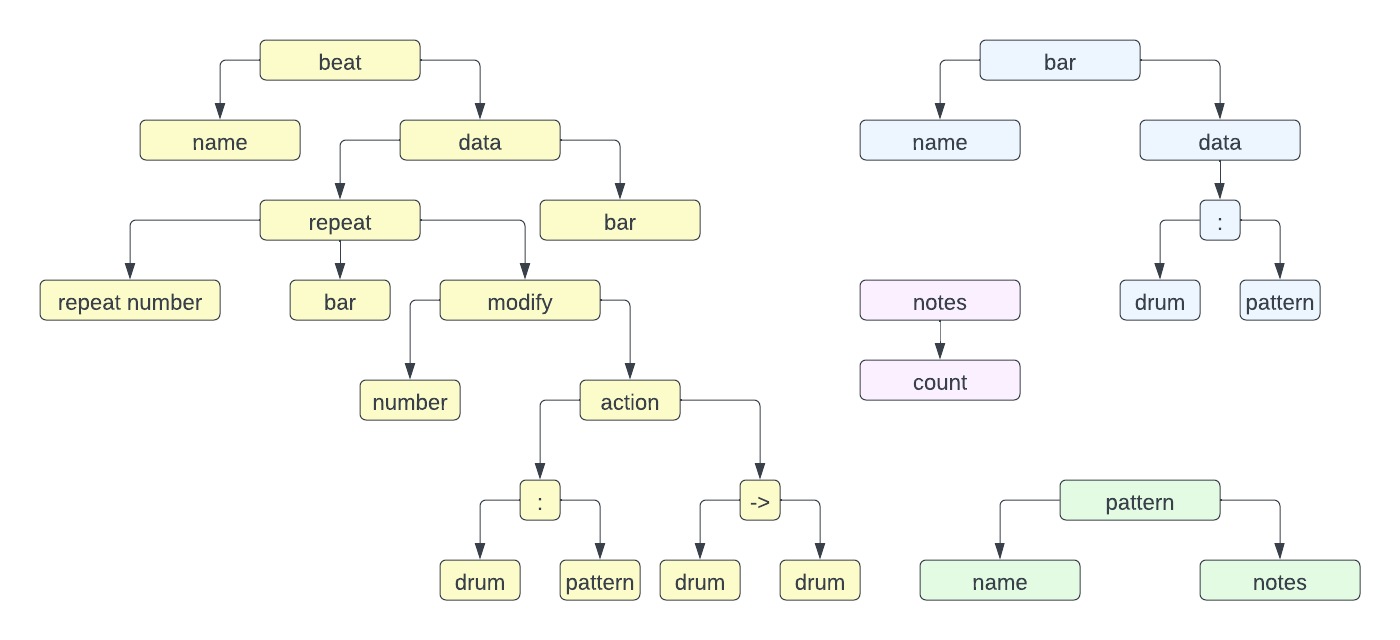
\includegraphics[scale=0.8]{Blank diagram.png}
    
    \item 


	AST for example 1:
    
    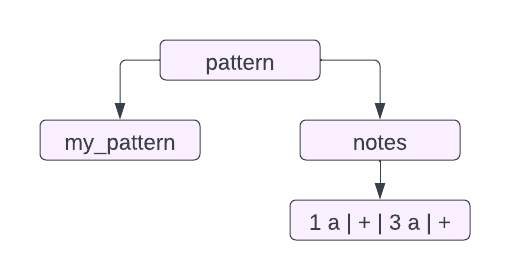
\includegraphics[scale=0.8]{Copy of Blank diagram-2.png}


	AST for example 2:
    
    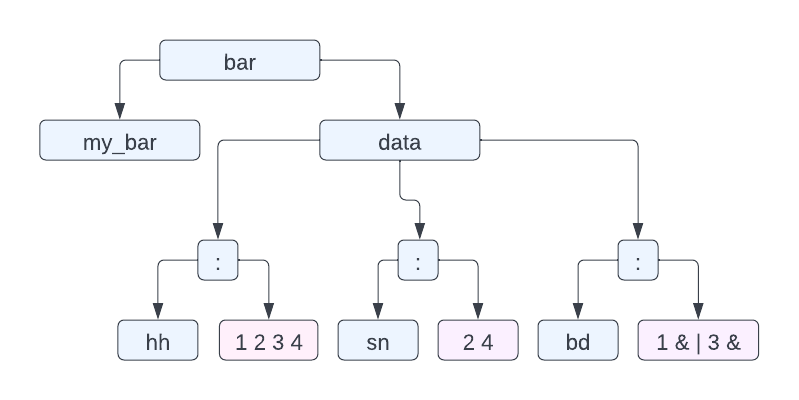
\includegraphics[scale=0.8]{Copy of Copy of Blank diagram.png}

	AST for example 3: (note that I've omitted the implementation of "my bar" as it is similar to example 2)
    
    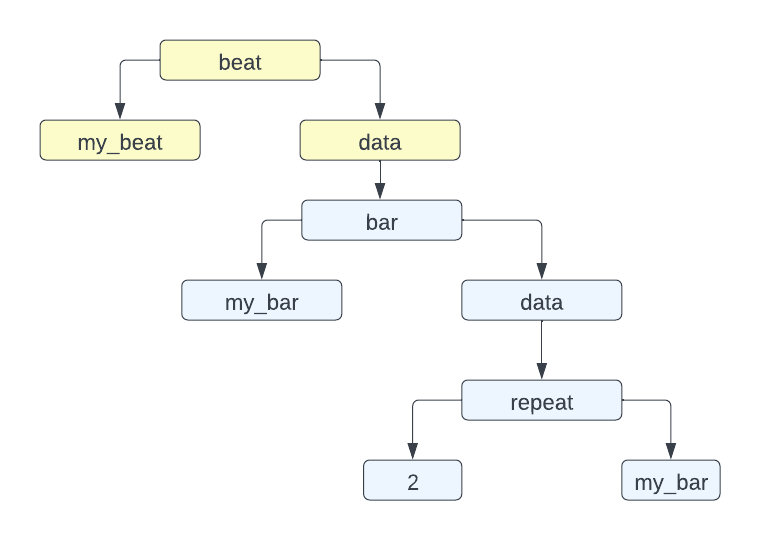
\includegraphics[scale=0.8]{Copy of Blank diagram.png}


    \item 
        \begin{enumerate}[A.]
        \item The programs in 1 e + a do not read any input.
        \item The output is a txt file which contains abc notation code.
        \item Evalution of the program illustrated by example 2. First we evaluate the left branch, which is name
		of the bar. The we evaluate the right branch which contains actions as children. Each action has a drum name 
		as the left node and a pattern as the right node. We first evaluate the drum, and then the pattern and assign
		the pattern to the drum. We continue doing so until we evaluate every action. 

		
		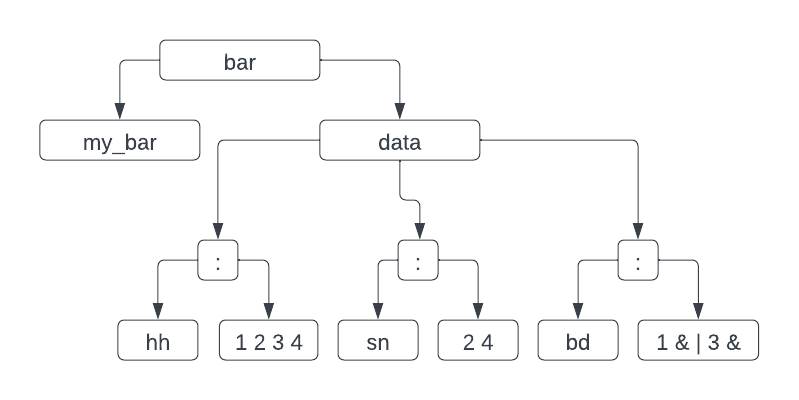
\includegraphics[scale=0.6]{Copy of Copy of Blank diagram-9.png}
		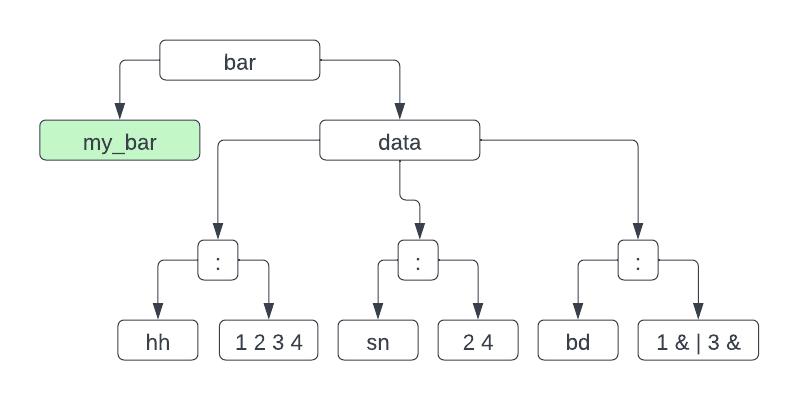
\includegraphics[scale=0.6]{Copy of Copy of Blank diagram-10.png}
		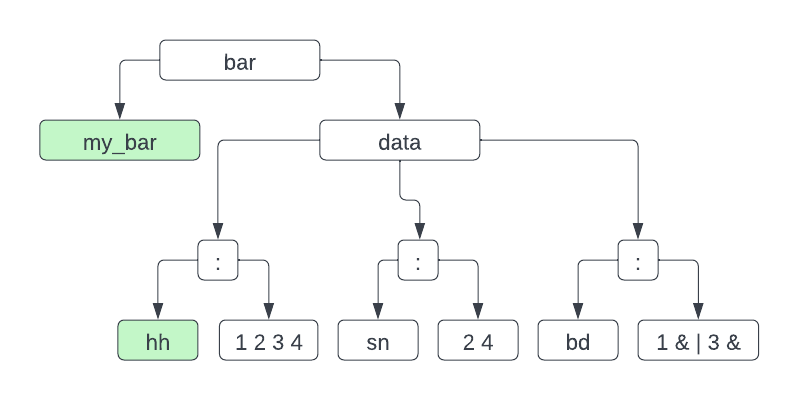
\includegraphics[scale=0.6]{Copy of Copy of Blank diagram-11.png}
		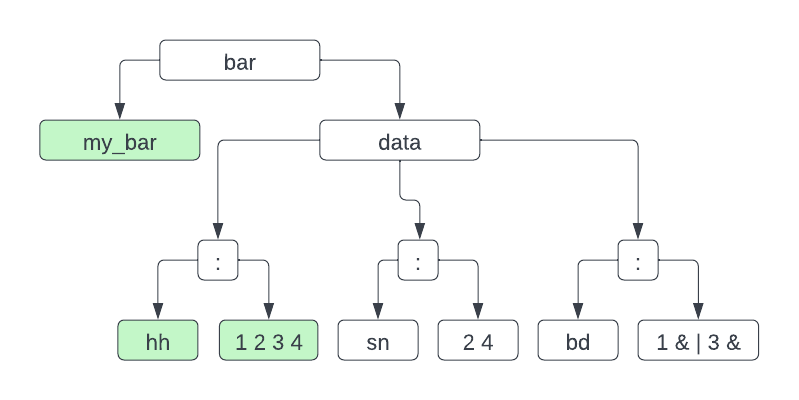
\includegraphics[scale=0.6]{Copy of Copy of Blank diagram-12.png}
		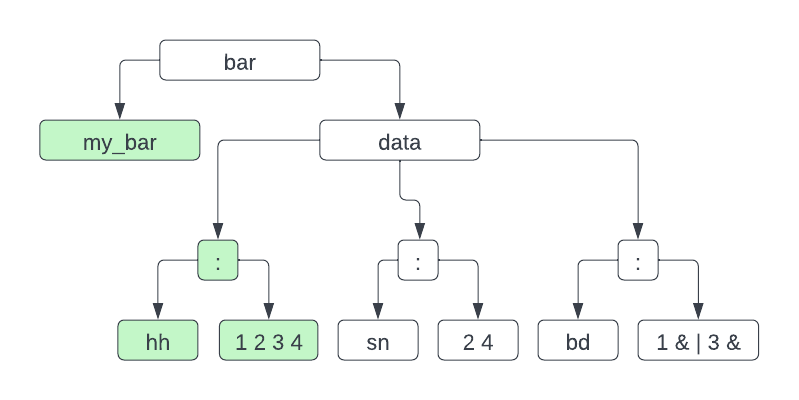
\includegraphics[scale=0.6]{Copy of Copy of Blank diagram-13.png}
		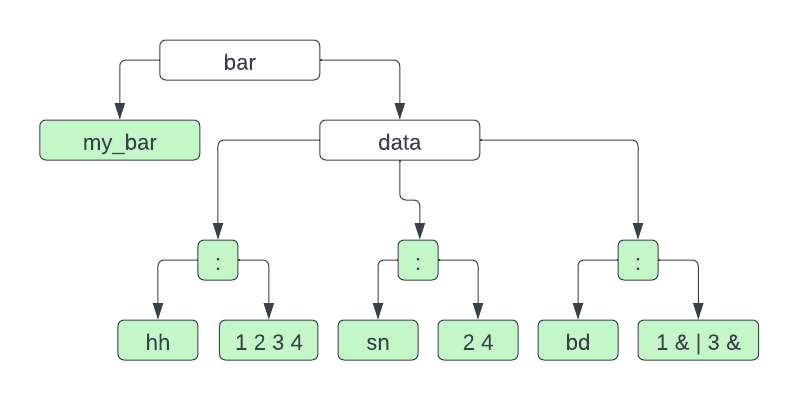
\includegraphics[scale=0.6]{Copy of Copy of Blank diagram-14.png}
		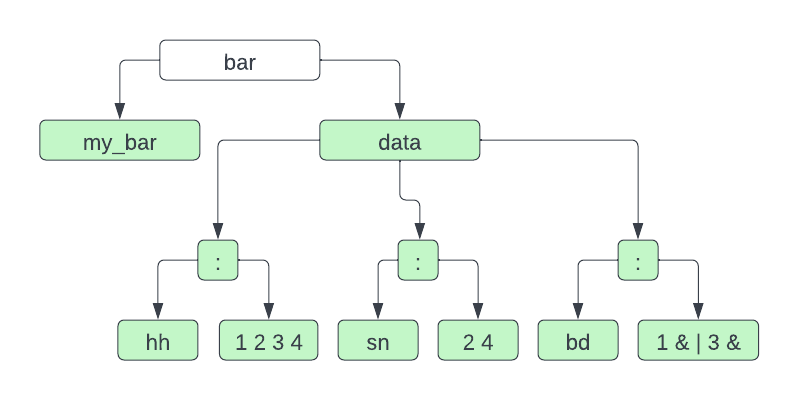
\includegraphics[scale=0.6]{Copy of Copy of Blank diagram-15.png}
		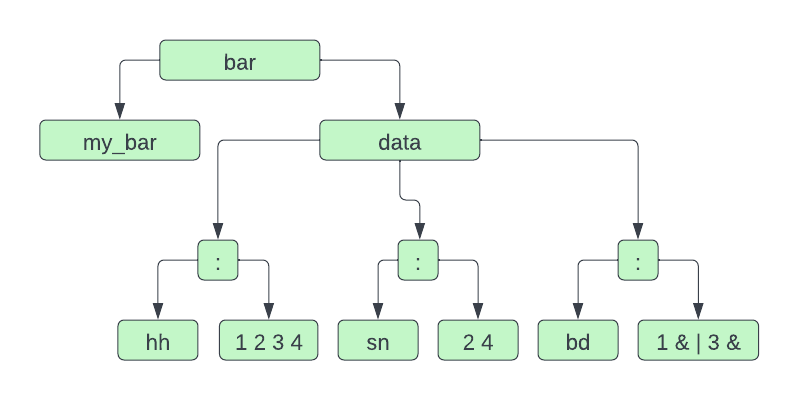
\includegraphics[scale=0.6]{Copy of Copy of Blank diagram-16.png}


        \end{enumerate}
    
\end{enumerate}


\section{Remaining Work}
1. Add a metronome feature to the webapp \\
2. Add a count-in feature to the webapp \\
3. Add a \\
4. Add support for time signatures other than 4/4 \\ 
5. Add support for division of beats other that 1/16 \\
6. Add constant variables\\

% DO NOT DELETE ANYTHING BELOW THIS LINE
\end{document}